\section{Hölder Table Function}
\label{sec:app:test:holder}
  The \emph{Hölder Table function} is a two-dimensional real-valued function
  employed in various branches of mathematical analysis.
  Due to its intriguing properties and complex topography, it serves as a
  valuable tool for function approximation and numerical analysis studies. 

  \begin{definition}[Hölder Table function]
  \label{def:app:test:holder}
    The \emph{Hölder Table function}, designated as \(f:\: \mathbb{R}^2 \to
    \mathbb{R}\), is described by the equation

    \begin{equation}
      \label{eq:app:test:holder}
      f(x,\, y) = -\left|
        \sin(x)\cos(y)\exp\left(
          \left|1 - \frac{\sqrt{x^2 + y^2}}{\pi}\right|
        \right)
      \right|
    \end{equation}

    This function is defined for \(-10 \leq x,\, y \leq 10\).
  \end{definition}

  The Hölder Table function peaks globally at \(f(x^*,\, y^*) = 19.208\,5\) for
  \(x^* = \pm 8.05502\) and \(y^* = \pm 9.66459\).
  Its intricately structured landscape can be vividly illustrated through
  contour and surface plots, as depicted in \vref{fig:app:test:holder}.

  \begin{figure}[ht!]
    \centering
    \begin{subfigure}[b]{0.45\textwidth}
      \centering
      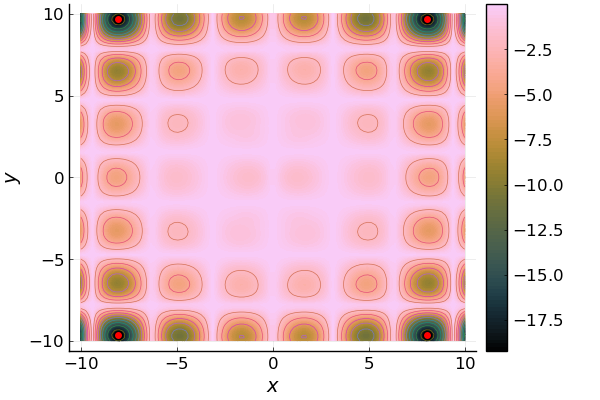
\includegraphics[width=\textwidth]
        {img/test_functions/holder_table_contour.png}
      \caption{
        Contour visualization of the Hölder Table function.
        The global minimum points are denoted by red dots.
      }
      \label{fig:app:test:holder:contour}
    \end{subfigure}
    \hfill
    \begin{subfigure}[b]{0.45\textwidth}
      \centering
      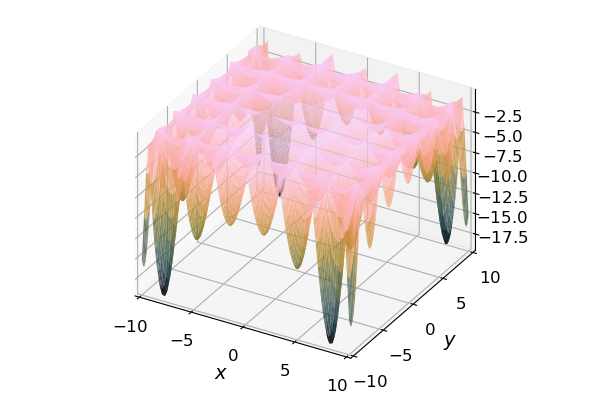
\includegraphics[width=\textwidth]
        {img/test_functions/holder_table_surface.png}
      \caption{
        Three-dimensional surface representation of the Hölder Table function.
      }
      \label{fig:app:test:holder:surface}
    \end{subfigure}
    \caption{
      The Complex Topography of the Hölder Table Function: Contour and Surface
      Representations
    }
    \label{fig:app:test:holder}
  \end{figure}
